\documentclass{standalone}
\usepackage[utf8]{inputenc}
\usepackage{tikz}
\usepackage{bm}
\usetikzlibrary{calc,patterns,decorations.pathmorphing,decorations.markings}
\usepackage{bm}


\def\mycolorv{black}
\def\mycolore{black}
\def\FF{\mathbf{F}}
\def\FFe{\mathbf{F}^\mathrm{e}}
\def\FFi{\mathbf{F}^\mathrm{i}}
\def\FFve{\mathbf{F}^\mathrm{ve}}
\def\FFvp{\mathbf{F}^\mathrm{vp}}
\def\PsiE{\Psi^{\mathrm{E}}}
\def\PsiV{\Psi^{\mathrm{i}}}

\begin{document}

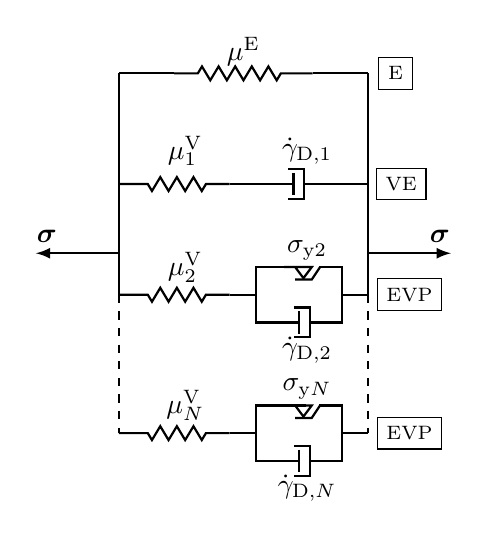
\begin{tikzpicture}
\tikzstyle{spring}=[thick,decorate,decoration={zigzag,pre length=0.3cm,post length=0.3cm,segment length=6}]
\tikzstyle{damper}=[thick,decoration={markings,
  mark connection node=dmp,
  mark=at position 0.5 with
  {
    \node (dmp) [thick,inner sep=0pt,transform shape,rotate=-90,minimum width=10pt,minimum height=3pt,draw=none] {};
    \draw [thick, color=\mycolorv] ($(dmp.north east)+(2pt,0)$) -- (dmp.south east) -- (dmp.south west) -- ($(dmp.north west)+(2pt,0)$);
    \draw [thick, color=\mycolorv] ($(dmp.north)+(0,-4pt)$) -- ($(dmp.north)+(0,4pt)$);
  }
}, decorate]
\tikzstyle{yield}=[thick,decoration={markings,
  mark connection node=yld,
  mark=at position 0.5 with
  {
    \node (yld) [thick,inner sep=0pt,transform shape,rotate=-90,minimum width=15pt,minimum height=12pt,draw=none] {};
    \draw [thick, color=\mycolorv] ($(yld.north)+(0,0)$) -- ($(yld.north)+(-4pt,0)$) -- ($(yld.north)+(-10pt,0)$) -- ($(yld.north)+(-7pt,4pt)$) -- ($(yld.north)+(-4pt,0)$);
    \draw [thick, color=\mycolorv] ($(yld.north)+(-4pt,4.5pt)$) -- ($(yld.north)+(-10pt,4.5pt)$) -- ($(yld.north)+(-13pt,0pt)$);
  }
}, decorate]
\tikzstyle{vp}=[thick,decoration={markings,
  mark connection node=vp,
  mark=at position 0.5 with
  {
    \node (vp) [thick,inner sep=0pt,transform shape,rotate=-90,minimum width=15pt,minimum height=30pt,draw=none] {};
    \draw [thick, color=\mycolorv] ($(vp.north)+(-18pt,-10pt)$) -- ($(vp.north)+(0pt,-10pt)$) -- ($(vp.north)+(0pt,10pt)$) -- ($(vp.north)+(-15pt,10pt)$);
    \draw [damper] ($(vp.north)+(-20pt,10pt)$) -- ($(vp.north)+(-15pt,10pt)$);
    \draw [yield] ($(vp.north)+(-25pt,-10pt)$) -- ($(vp.north)+(-8pt,-10pt)$);
    \draw [thick, color=\mycolorv] ($(vp.north)+(-25pt,-10pt)$) -- ($(vp.north)+(-31pt,-10pt)$) -- ($(vp.north)+(-31pt,10pt)$) -- ($(vp.north)+(-20pt,10pt)$);
  }
}, decorate]
\tikzstyle{ground}=[fill,pattern=north east lines,draw=none,minimum width=0.75cm,minimum height=0.3cm]

\coordinate (left1) at (0,0) {};
\path (left1) + (0, -40pt) coordinate (left2);
\path (left2) + (0, -40pt) coordinate (left3);
\path (left3) + (0, -50pt) coordinate (left4);
\path (left1) + (0, -65pt) coordinate (leftmid);

\path (left1) + (90pt, 0) coordinate (right1);
\path (right1) + (0, -40pt) coordinate (right2);
\path (right2) + (0, -40pt) coordinate (right3);
\path (right3) + (0, -50pt) coordinate (right4);
\path (right1) + (0, -65pt) coordinate (rightmid);

\path (left1) + (20pt, 0) coordinate (midleft1);
\path (right1) + (-20pt, 0) coordinate (midright1);
\path (left2) + (40pt, 0) coordinate (mid2);
\path (left3) + (40pt, 0) coordinate (mid3);
\path (left4) + (40pt, 0) coordinate (mid4);

\path (left3) + (0,-20pt) coordinate (left3r);
\path (right3) + (0,-20pt) coordinate (right3r);

\draw [-, thick] (left1) -- (left3);
\draw [-, thick] (right1) -- (right3);
\draw [-, thick, dashed] (left3) -- (left4);
\draw [-, thick, dashed] (right3) -- (right4);

\draw [thick, color=\mycolore] (midleft1) -- (left1);
\draw [thick, color=\mycolore] (right1) -- (midright1);

\draw [spring, color=\mycolore] (midleft1) -- (midright1);
\draw [spring, color=\mycolorv] (mid2) -- (left2);
\draw [damper, color=\mycolorv] (right2) -- (mid2);

\draw [spring, color=\mycolorv] (mid3) -- (left3);
\draw [vp, color=\mycolorv] (right3) -- (mid3);

\draw [spring, color=\mycolorv] (mid4) -- (left4);
\draw [vp, color=\mycolorv] (right4) -- (mid4);



\node (A) [yshift=8pt, xshift=45pt, color=\mycolorv] at (left1) {$\mu^{\mathrm{E}}$};
\node (B1) [yshift=12pt, xshift=-16pt, color=\mycolorv] at (mid2) {$\mu^{\mathrm{V}}_1$};
\node (B2) [yshift=12pt, xshift=28pt, color=\mycolorv] at (mid2) {$\dot{\gamma}_{\mathrm{D},1}$};
\node (C1) [yshift=10pt, xshift=-16pt, color=\mycolorv] at (mid3) {$\mu^{\mathrm{V}}_2$};
\node (C2) [yshift=16pt, xshift=28pt, color=\mycolorv] at (mid3) {${\sigma}_{\mathrm{y}2}$};
\node (C3) [yshift=-20pt, xshift=28pt, color=\mycolorv] at (mid3) {$\dot{\gamma}_{\mathrm{D},2}$};
\node (D1) [yshift=10pt, xshift=-16pt, color=\mycolorv] at (mid4) {$\mu^{\mathrm{V}}_N$};
\node (D2) [yshift=16pt, xshift=28pt, color=\mycolorv] at (mid4) {${\sigma}_{\mathrm{y}N}$};
\node (D3) [yshift=-20pt, xshift=28pt, color=\mycolorv] at (mid4) {$\dot{\gamma}_{\mathrm{D},N}$};

\node (E) [draw, xshift=10pt] at (right1) {\scriptsize E};
\node (VE) [draw, xshift=12pt] at (right2) {\scriptsize VE};
\node (VP1) [draw, xshift=15pt] at (right3) {\scriptsize EVP};
\node (VP2) [draw, xshift=15pt] at (right4) {\scriptsize EVP};



\draw [-latex,thick] (leftmid) -- +(-30pt, 0);
\draw [-latex,thick] (rightmid) -- +(30pt, 0);
\node (Fu) [yshift=6pt, xshift=-26pt] at (leftmid) {$\bm{\sigma}$};
\node (Fd) [yshift=6pt, xshift=26pt] at (rightmid) {$\bm{\sigma}$};

\end{tikzpicture}

\end{document}